\documentclass{article}
\usepackage{pgfplots}
\usepackage{tikz}
\usetikzlibrary{patterns}
\usetikzlibrary{positioning}

\begin{document}

\begin{figure}
    \centering
    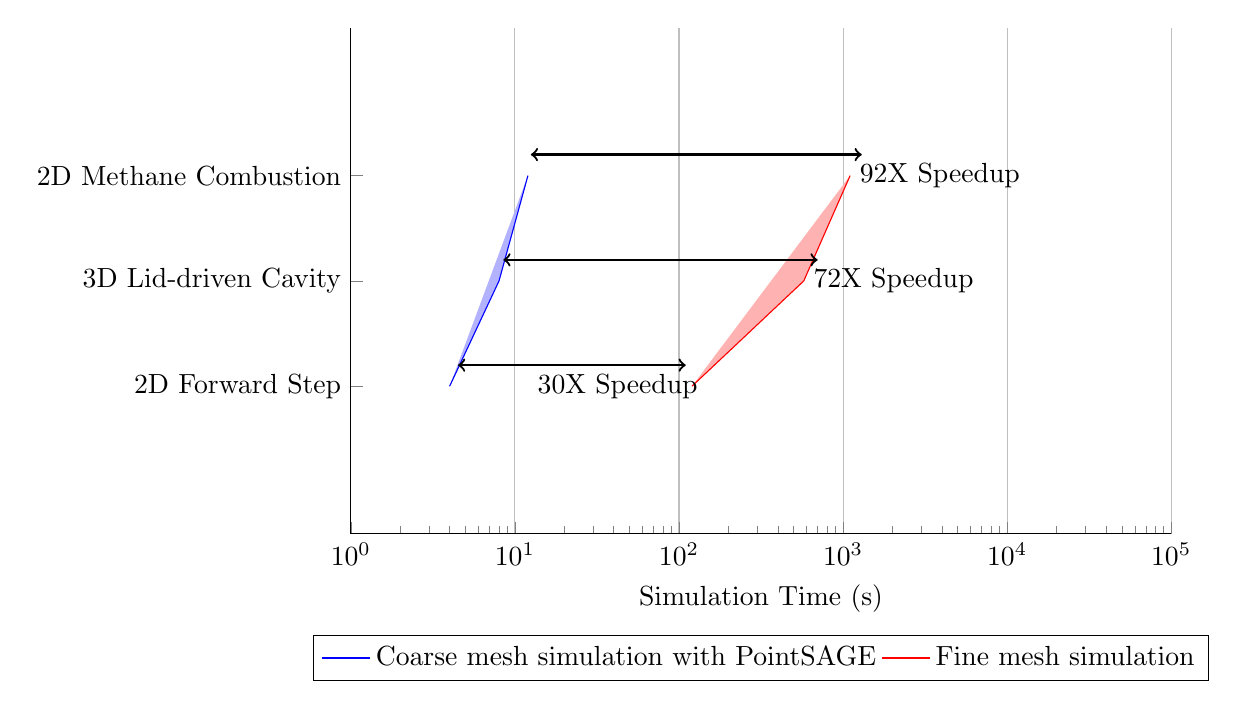
\begin{tikzpicture}
        \begin{axis}[
            xmode=log,
            width=12cm,
            height=8cm,
            xlabel={Simulation Time (s)},
            ylabel={},
            ytick={1, 2, 3},
            yticklabels={2D Forward Step, 3D Lid-driven Cavity, 2D Methane Combustion},
            xmin=1, xmax=100000,
            ymin=0.5, ymax=3.5,
            axis y line*=left,
            axis x line*=bottom,
            xmajorgrids=true,
            ymajorgrids=false,
            enlarge y limits=0.3,
            legend style={at={(0.5,-0.2)}, anchor=north, legend columns=-1},
            bar width=0.5cm,
        ]
        \addplot[draw=blue, fill=blue!30] coordinates {(4,1) (8,2) (12,3)};
        \addplot[draw=red, fill=red!30] coordinates {(120,1) (576,2) (1104,3)};
        
        \legend{Coarse mesh simulation with PointSAGE, Fine mesh simulation}

        \node[anchor=west] at (axis cs:12,1) {30X Speedup};
        \node[anchor=west] at (axis cs:576,2) {72X Speedup};
        \node[anchor=west] at (axis cs:1104,3) {92X Speedup};

        \draw[<->, thick] (axis cs:4.5,1.2) -- (axis cs:110,1.2);
        \draw[<->, thick] (axis cs:8.5,2.2) -- (axis cs:700,2.2);
        \draw[<->, thick] (axis cs:12.5,3.2) -- (axis cs:1300,3.2);

        \end{axis}
    \end{tikzpicture}
\end{figure}

\end{document}